%%%%%%%%%%%%%%%%%%%%%%%%%%%%%%%%%%%%%%%%%%%%%%%%%%%%%%%%%%%%%%%%%%%%%%%%%%%%%%%
\begin{frame}
 %\frametitle{Introduction}
 \vskip-0.1in
 \begin{figure}
  \begin{center}
   
\includegraphics[height=0.15\textheight]{logos/ForWarn_Logo}
   \hfill
   
\includegraphics[width=0.14\textheight]{logos/USFS_Logo}
   \hfill
   
\includegraphics[width=0.17\textheight]{logos/NASA_Logo}
   \hfill
   
\includegraphics[width=0.15\textheight]{logos/DOE_Logo}
   \hfill
   
\includegraphics[width=0.15\textheight]{logos/DOI_Logo}
  \end{center}
 \end{figure}
 \vskip-0.1in
  The USDA Forest Service, NASA Stennis Space Center, DOE Oak Ridge National Laboratory, and DOI Eros Data Center have created a system to monitor threats to U.S. forests and wildlands:
 \begin{itemize}
  \item {\color{red}Tier 1: Strategic} --- The \emph{ForWarn} system that routinely monitors wide areas at coarser resolution, repeated frequently --- a \emph{change detection system} to produce alerts or warnings for particular locations may be of interest
  \item{\color{red}Tier 2: Tactical} --- Finer resolution airborne overflights and ground inspections of areas of potential interest --- \emph{Aerial Detection Survey (ADS)} monitoring to determine if such warnings become alarms
 \end{itemize}
 Tier 2 was in place and managed by the USDA Forest Service, but Tier 1 was needed to optimally direct its labor-intensive efforts and discover new threats sooner.
\end{frame}
%%%%%%%%%%%%%%%%%%%%%%%%%%%%%%%%%%%%%%%%%%%%%%%%%%%%%%%%%%%%%%%%%%%%%%%%%%%%%%%

%%%%%%%%%%%%%%%%%%%%%%%%%%%%%%%%%%%%%%%%%%%%%%%%%%%%%%%%%%%%%%%%%%%%%%%%%%%%%%%
\begin{frame}
 \frametitle{Design Plan for the \textit{ForWarn} Early Warning System}
 \begin{figure}
  \begin{center}
   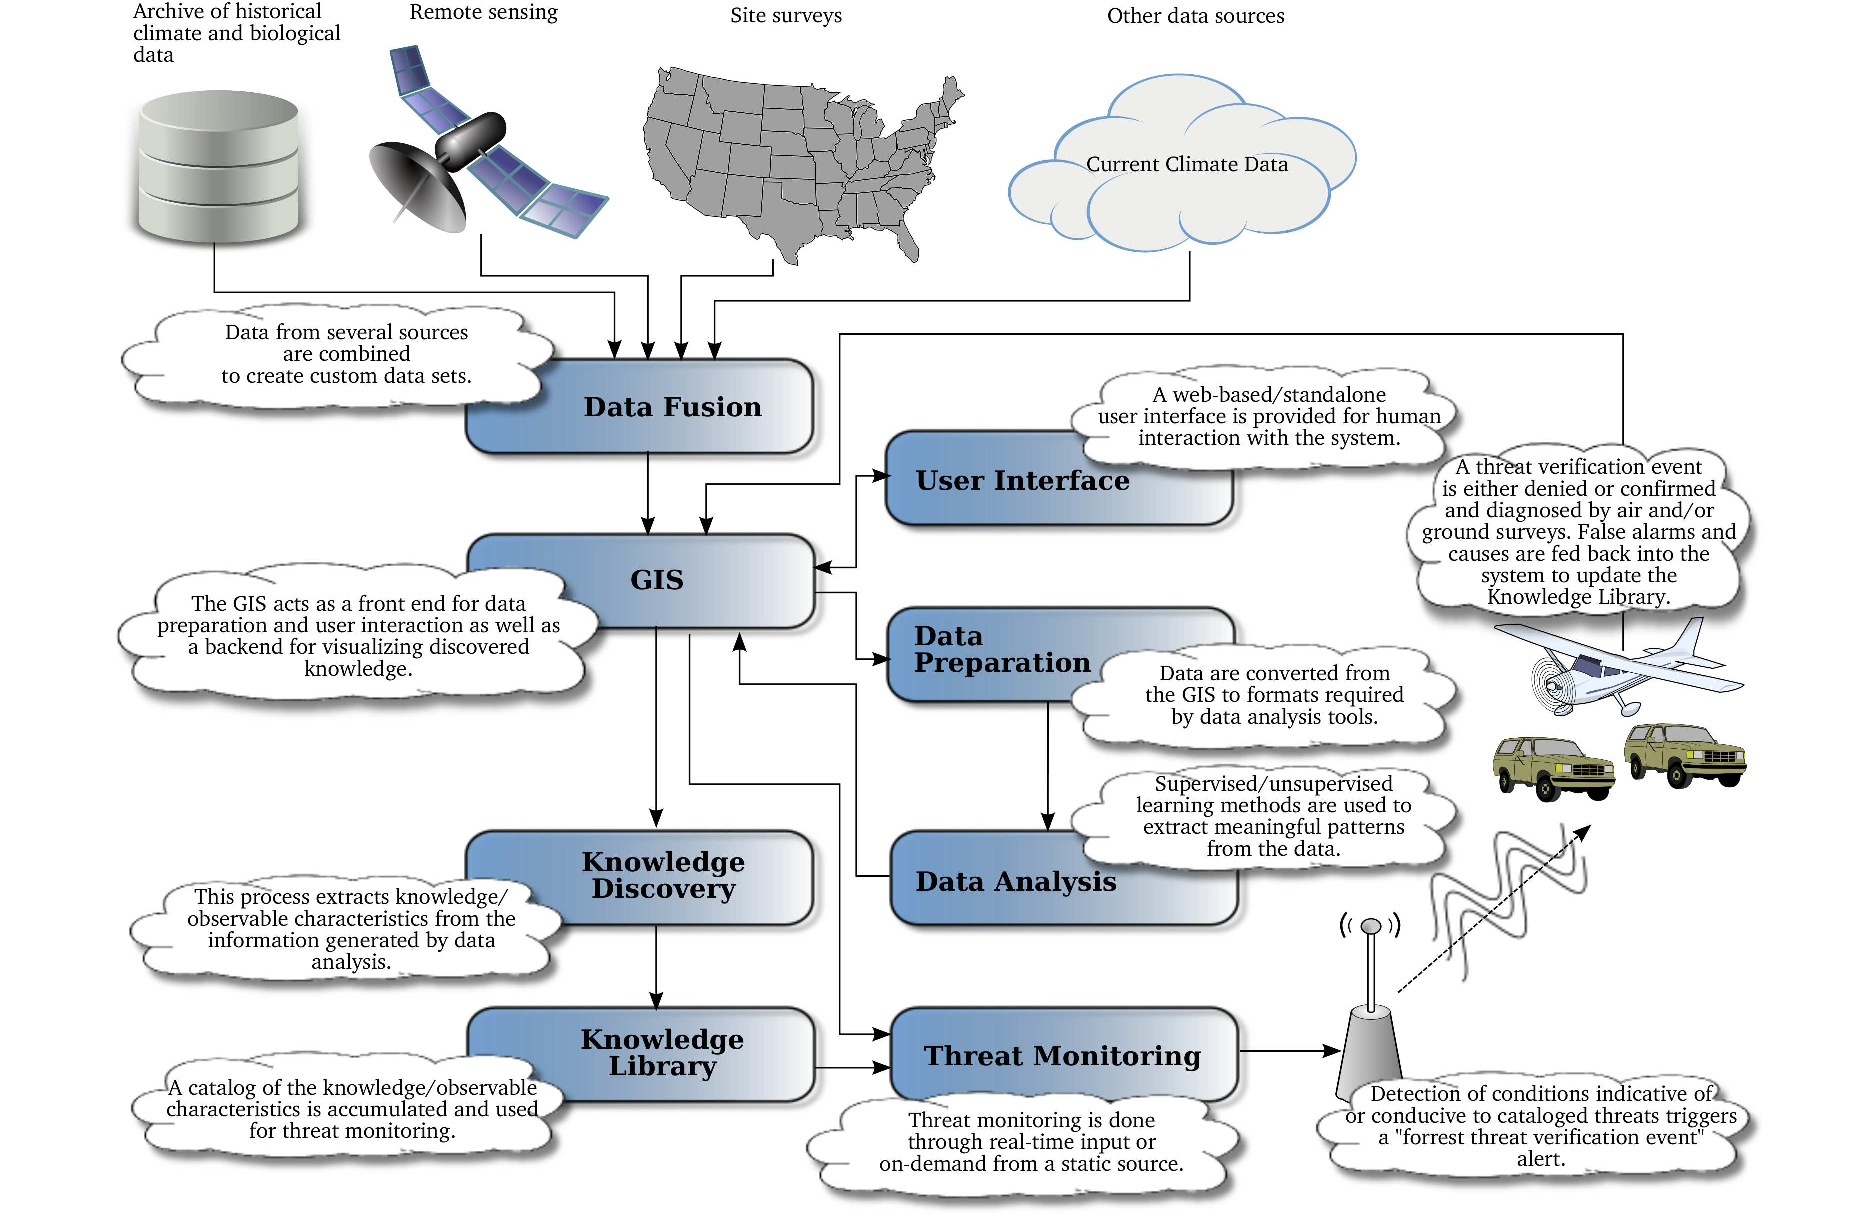
\includegraphics[width=\textwidth]{figures/EWS}
  \end{center}
  %\caption{Early Warning System}
  \label{fig:EWS}
 \end{figure}
\end{frame}
%%%%%%%%%%%%%%%%%%%%%%%%%%%%%%%%%%%%%%%%%%%%%%%%%%%%%%%%%%%%%%%%%%%%%%%%%%%%%%%

%%%%%%%%%%%%%%%%%%%%%%%%%%%%%%%%%%%%%%%%%%%%%%%%%%%%%%%%%%%%%%%%%%%%%%%%%%%%%%%
\begin{frame}
 \frametitle{Normalized Difference Vegetation Index (NDVI)}
 \begin{itemize}
  \item NDVI exploits the strong differences in plant reflectance between red and near-infrared wavelengths to provide a measure of {\color{DarkGreen}``greenness''} from remote sensing measurements. 
  \begin{equation}
   \textnormal{NDVI} = \frac{\left(\sigma_\textnormal{nir} - \sigma_\textnormal{red}\right)}{\left(\sigma_\textnormal{nir} + \sigma_\textnormal{red}\right)}
  \end{equation}
  \item These spectral reflectances are ratios of reflected over incoming radiation, $\sigma = {I_r} / {I_i}$, hence they take on values between $0.0$ and $1.0$.  As a result, NDVI varies between $-1.0$ and $+1.0$.
  \item Dense vegetation cover is $0.3$--$0.8$, soils are about $0.1$--$0.2$, surface water is near $0.0$, and clouds and snow are negative.
 \end{itemize}
\end{frame}
%%%%%%%%%%%%%%%%%%%%%%%%%%%%%%%%%%%%%%%%%%%%%%%%%%%%%%%%%%%%%%%%%%%%%%%%%%%%%%%

%%%%%%%%%%%%%%%%%%%%%%%%%%%%%%%%%%%%%%%%%%%%%%%%%%%%%%%%%%%%%%%%%%%%%%%%%%%%%%%
{
\usebackgroundtemplate{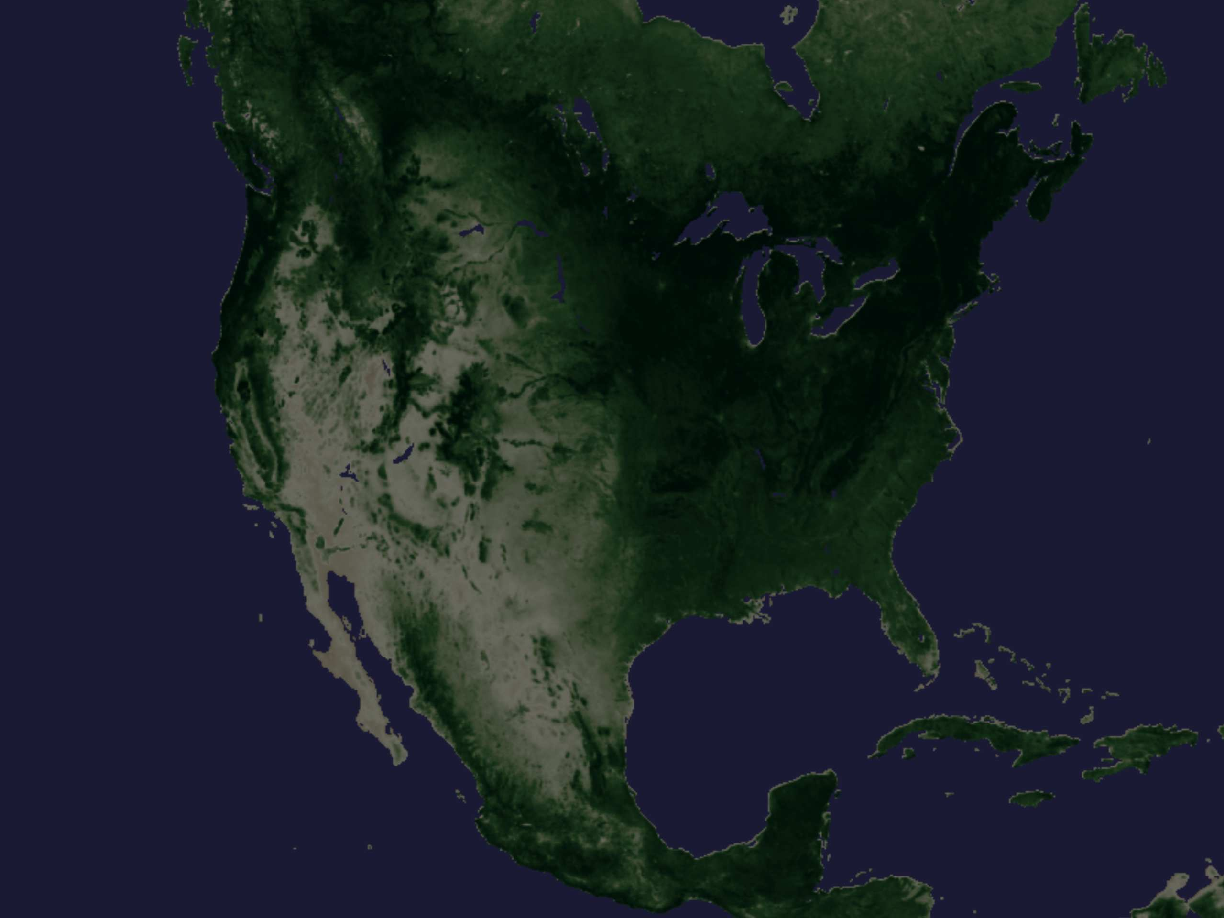
\includegraphics[width=\paperwidth]{figures/na_season0007}}
\begin{frame}
 \frametitle{MODIS MOD13 NDVI Product}
 \begin{itemize}\color{white}
  \item The Moderate Resolution Imaging Spectroradiometer (MODIS) is a key instrument aboard the Terra (EOS AM, N$\rightarrow$S) and Aqua (EOS PM, S$\rightarrow$N) satellites.
  \item Both view the entire surface of Earth every 1 to 2 days, acquiring data in 36 spectral bands.
  \item The MOD 13 product provides Gridded Vegetation Indices (NDVI and EVI) to characterize vegetated surfaces.
  \item Available are 6 products at varying spatial (250~m, 1~km, 0.05$^\circ$) and temporal (16-day, monthly) resolutions.
  \item The Terra and Aqua products are staggered in time so that a new product is available every 8 days.
  \item Results shown here are derived from the 8-day Terra+Aqua  MODIS product at 250~m resolution, processed by NASA Stennis Space Center.
 \end{itemize}
\end{frame}
}
%%%%%%%%%%%%%%%%%%%%%%%%%%%%%%%%%%%%%%%%%%%%%%%%%%%%%%%%%%%%%%%%%%%%%%%%%%%%%%%

%%%%%%%%%%%%%%%%%%%%%%%%%%%%%%%%%%%%%%%%%%%%%%%%%%%%%%%%%%%%%%%%%%%%%%%%%%%%%%%
\begin{frame}
 \vskip-0.10in
 \begin{columns}[c]
  \column{0.66\textwidth}
  \begin{itemize}
   \item {\color{blue}Phenology} is the study of periodic plant and animal life cycle events and how these are influenced by seasonal and interannual variations in climate.
   \item \textit{ForWarn} is interested in deviations from the ``normal'' seasonal cycle of vegetation growth and senescence.
   \item NASA Stennis Space Center has developed a new set of National Phenology Datasets based on MODIS.
   \item Outlier/noise removal and temporal smoothing are performed, followed by curve-fitting and estimation of descriptive curve parameters.
  \end{itemize}

  \vskip0.1in
  \vbox{\scriptsize Up-looking photos of a scarlet oak showing the timing of leaf emergence in the spring~\citep{Hargrove_PERS_20091001}.}
  \column{0.33\textwidth}
  \begin{figure}
   \begin{center}
    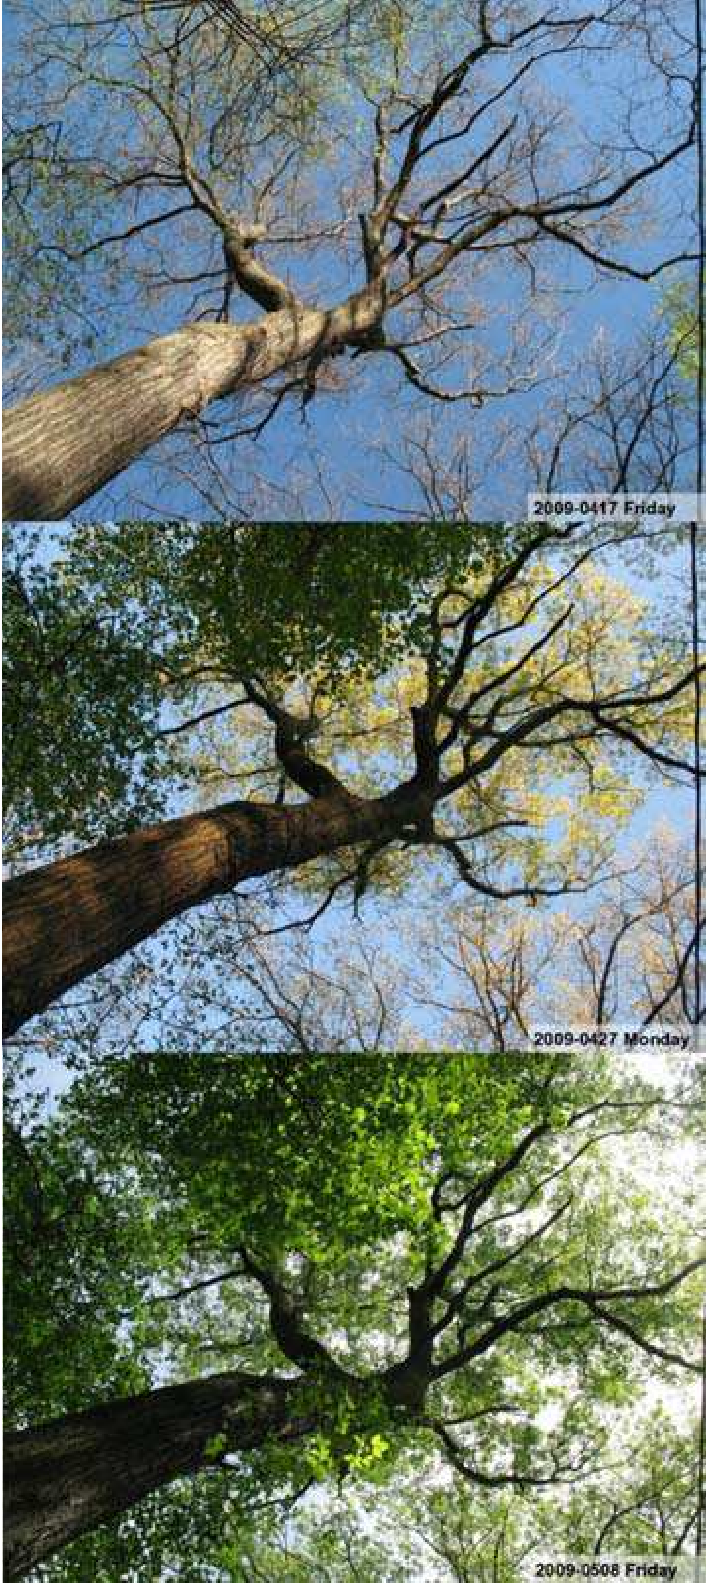
\includegraphics[width=\textwidth]{figures/up-looking_photos}
   \end{center}
   %\caption{Up-looking photos~\cite{Hargrove_PERS_20091001}}
   \label{fig:up-looking_photos}
  \end{figure}
 \end{columns}
\end{frame}
%%%%%%%%%%%%%%%%%%%%%%%%%%%%%%%%%%%%%%%%%%%%%%%%%%%%%%%%%%%%%%%%%%%%%%%%%%%%%%%

%%%%%%%%%%%%%%%%%%%%%%%%%%%%%%%%%%%%%%%%%%%%%%%%%%%%%%%%%%%%%%%%%%%%%%%%%%%%%%%
\begin{frame}
 \frametitle{Annual Greenness Profile Through Time}
  \begin{center}
   \vskip-0.05in
   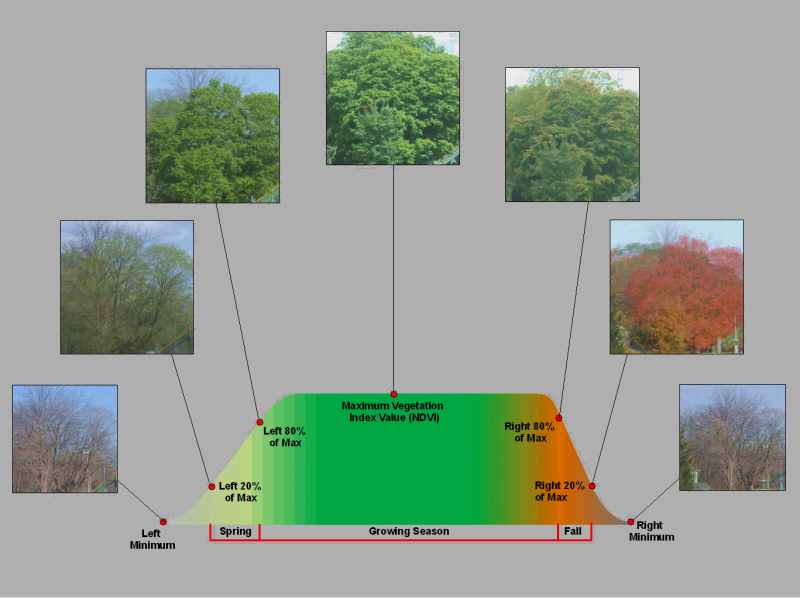
\includegraphics[width=0.92\textwidth]{figures/fancyprofile}
  \end{center}
\end{frame}
%%%%%%%%%%%%%%%%%%%%%%%%%%%%%%%%%%%%%%%%%%%%%%%%%%%%%%%%%%%%%%%%%%%%%%%%%%%%%%%

%%%%%%%%%%%%%%%%%%%%%%%%%%%%%%%%%%%%%%%%%%%%%%%%%%%%%%%%%%%%%%%%%%%%%%%%%%%%%%%
{\setbeamercolor{background canvas}{bg=black}
\begin{frame}
 \frametitle{MODIS Snapshots by Season -- Walker Branch}
  \begin{center}
   \vskip-0.12in
   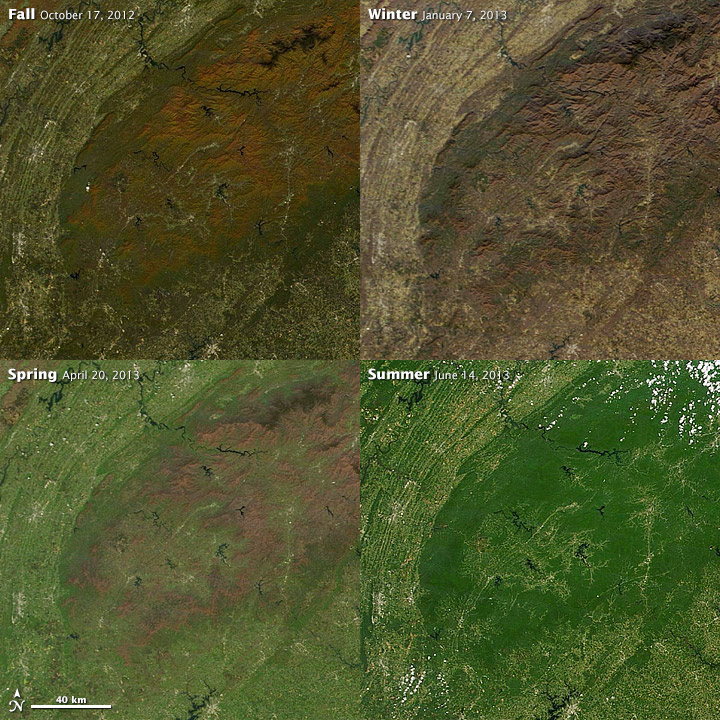
\includegraphics[width=0.72\textwidth]{figures/WalkerBranch_amo_seasons_2012-13.jpg}
  \end{center}
\end{frame}
}
%%%%%%%%%%%%%%%%%%%%%%%%%%%%%%%%%%%%%%%%%%%%%%%%%%%%%%%%%%%%%%%%%%%%%%%%%%%%%%%

%%%%%%%%%%%%%%%%%%%%%%%%%%%%%%%%%%%%%%%%%%%%%%%%%%%%%%%%%%%%%%%%%%%%%%%%%%%%%%%
\begin{frame}
 %\frametitle{PERS Cover}
 \vskip-0.10in
 \begin{columns}[c]
  \column{0.44\textwidth}{\small
  \begin{itemize}
   \item To detect vegetation disturbances, the current NDVI measurement is compared with the normal, expected baseline for the same location.
   \item Substantial decreases from the baseline represent potential disturbances.
   \item Any increases over the baseline may represent vegetation recovery.
   \item Maximum, mean, or median NDVI may provide a suitable baseline value.
  \end{itemize}
  }
  \vbox{\scriptsize
   June 10--23, 2009, NDVI is loaded into blue and green; maximum NDVI from 2001--2006 is loaded into red~\citep{Hargrove_PERS_20091001}.
  }
  \column{0.55\textwidth}
  \begin{figure}
   \begin{center}
    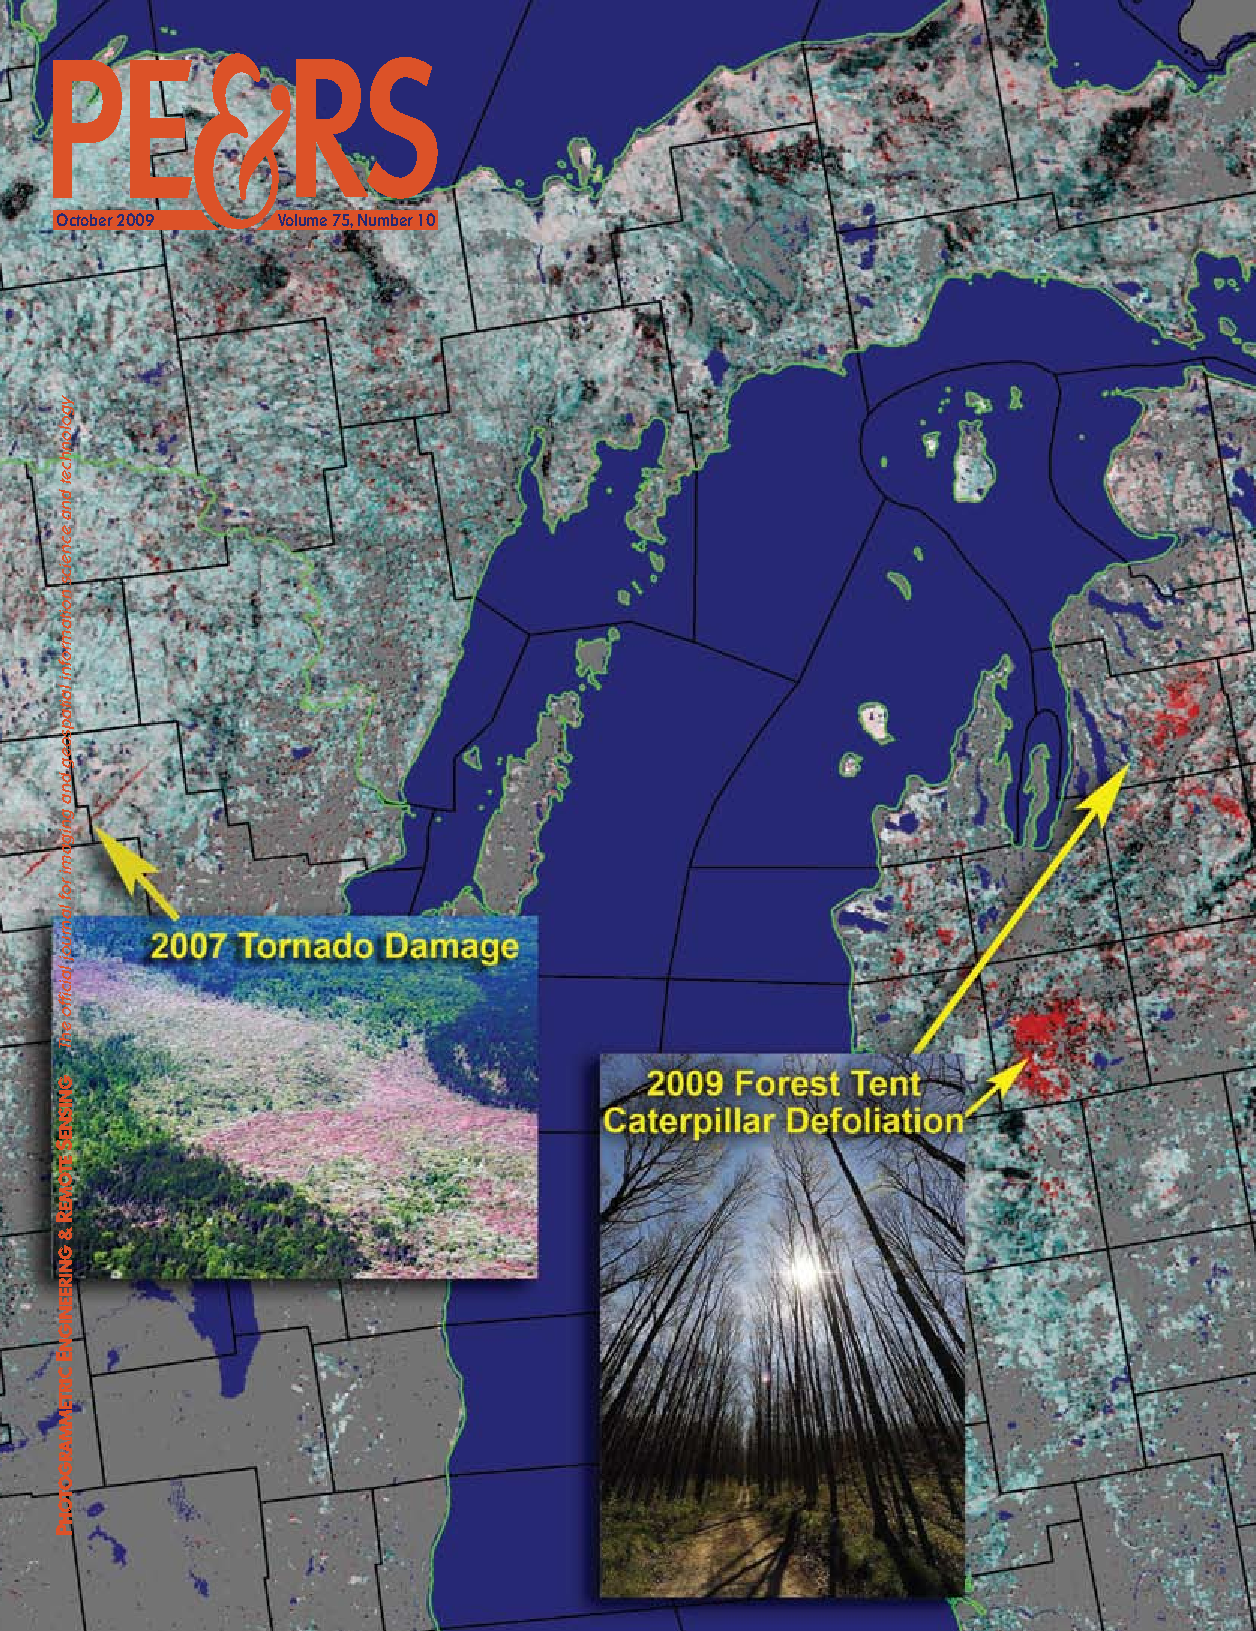
\includegraphics[width=\textwidth]{figures/Hargrove_PERS-Cover_20091001}
   \end{center}
   %\caption{Phenoregions}
   \label{fig:PERS_cover}
  \end{figure}
 \end{columns}
\end{frame}
%%%%%%%%%%%%%%%%%%%%%%%%%%%%%%%%%%%%%%%%%%%%%%%%%%%%%%%%%%%%%%%%%%%%%%%%%%%%%%%

%%%%%%%%%%%%%%%%%%%%%%%%%%%%%%%%%%%%%%%%%%%%%%%%%%%%%%%%%%%%%%%%%%%%%%%%%%%%%%%
\begin{frame}
 \frametitle{Three Hurricanes}
 \vskip-0.15in
 \begin{figure}
  \begin{center}
   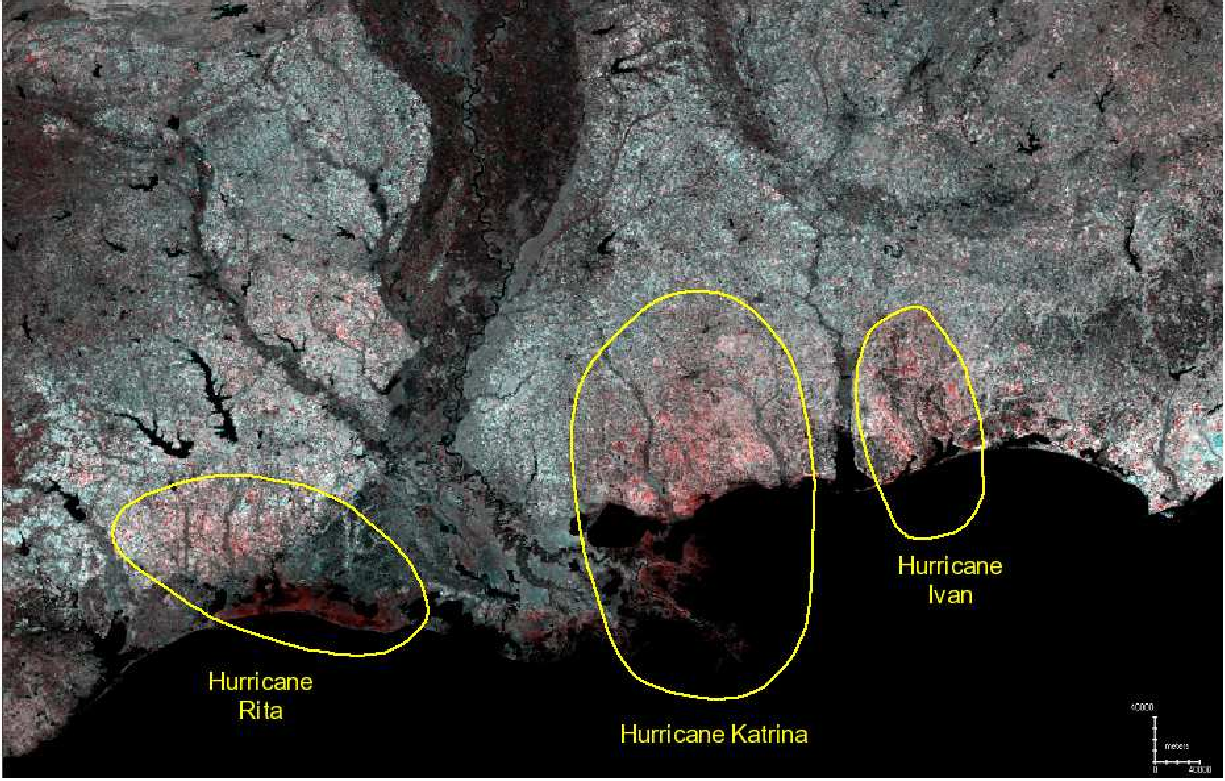
\includegraphics[width=0.87\textwidth]{figures/MODIS3hurricanes3} \\
   \vbox{\small Computed by assigning 2006 20\% left value to green \& blue, and 20\% left from 2004 to red~\citep{Hargrove_PERS_20091001}. Red depicts areas of reduced greenness, primarily east of storm tracks and in marshes.}
  \end{center}
  %\caption{Damage from three hurricanes.}
  \label{fig:MODIS3hurricanes3}
 \end{figure}
\end{frame}
%%%%%%%%%%%%%%%%%%%%%%%%%%%%%%%%%%%%%%%%%%%%%%%%%%%%%%%%%%%%%%%%%%%%%%%%%%%%%%%

%%%%%%%%%%%%%%%%%%%%%%%%%%%%%%%%%%%%%%%%%%%%%%%%%%%%%%%%%%%%%%%%%%%%%%%%%%%%%%%
\begin{frame}
 \frametitle{Arkansas Ozarks Ice Storm, Jan. 26--29, 2009}
 \vskip-0.15in
 \begin{figure}
  \begin{center}
   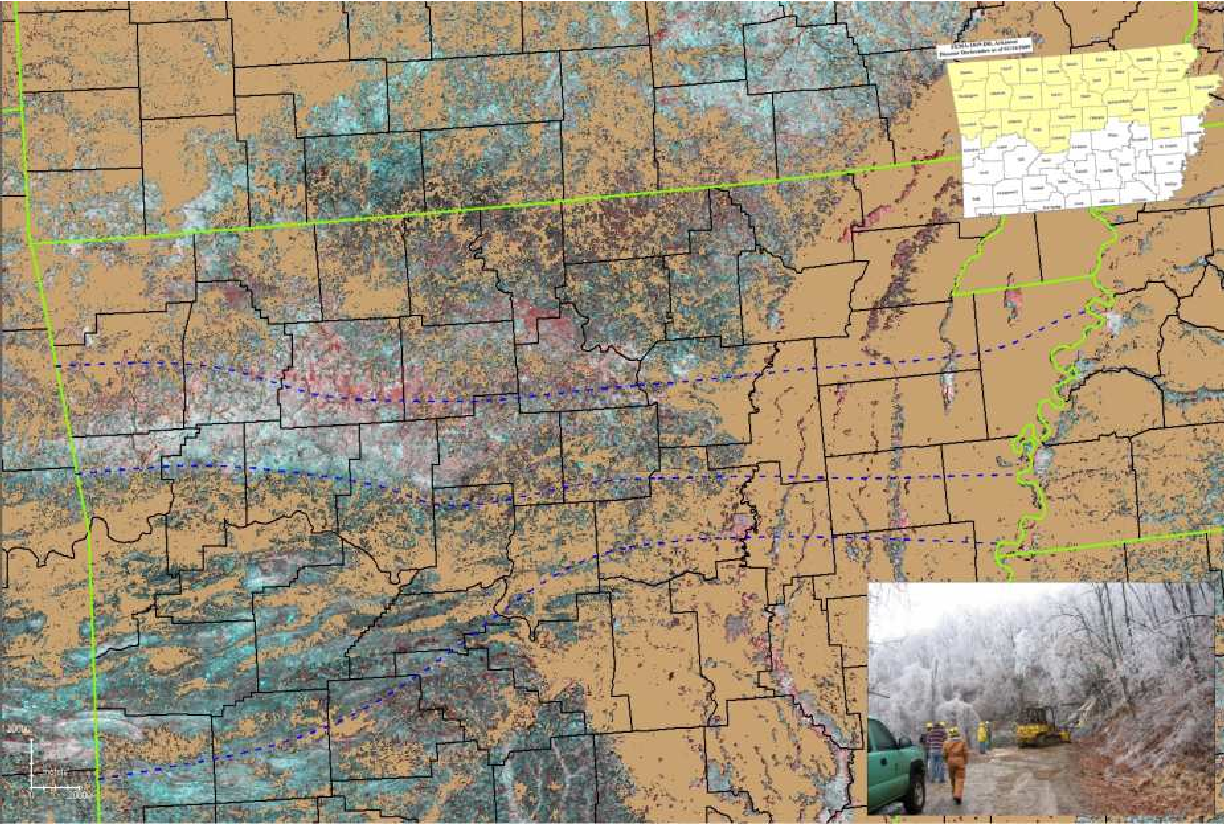
\includegraphics[width=0.85\textwidth]{figures/arkansasicestorm3slide} \\
   \vbox{\small Computed by assigning 2009 max NDVI for June 10--July 15 into blue \& green, and 2001--2006 max NDVI for June 10--July 27 into red.  Storm resulted in 35,000 without power and 18 fatalities.}
  \end{center}
  %\caption{Arkansas Ozarks Ice Storm}
  \label{fig:arkansasicestorm3slide}
 \end{figure}
\end{frame}
%%%%%%%%%%%%%%%%%%%%%%%%%%%%%%%%%%%%%%%%%%%%%%%%%%%%%%%%%%%%%%%%%%%%%%%%%%%%%%%

%%%%%%%%%%%%%%%%%%%%%%%%%%%%%%%%%%%%%%%%%%%%%%%%%%%%%%%%%%%%%%%%%%%%%%%%%%%%%%%
\begin{frame}
 \begin{center}
  \vskip-0.13cm
  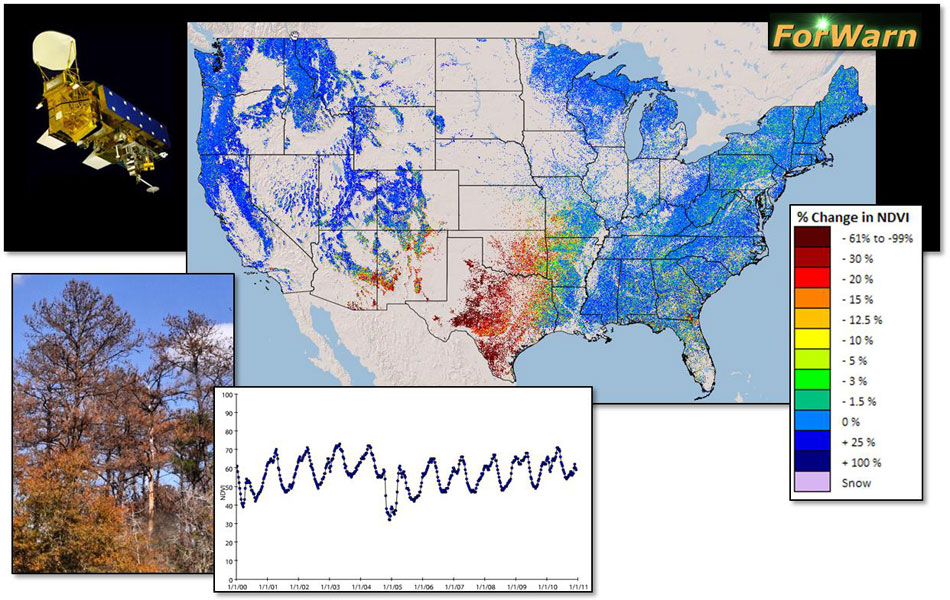
\includegraphics[width=0.95\textwidth]{figures/ForWarnUS.jpg}
 \end{center}
 \vskip-0.13cm
 \vbox{\footnotesize \textit{ForWarn} is a forest change recognition and tracking system that uses high-frequency, moderate resolution satellite data to provide near real-time forest change maps for the continental United States that are updated every eight days.  Maps and data products are available in the \textbf{Forest Change Assessment Viewer} at \url{http://forwarn.forestthreats.org/fcav/}}
\end{frame}
%%%%%%%%%%%%%%%%%%%%%%%%%%%%%%%%%%%%%%%%%%%%%%%%%%%%%%%%%%%%%%%%%%%%%%%%%%%%%%%

%%%%%%%%%%%%%%%%%%%%%%%%%%%%%%%%%%%%%%%%%%%%%%%%%%%%%%%%%%%%%%%%%%%%%%%%%%%%%%%
%\begin{frame}\small
% \begin{center}
%  \vskip-0.13cm
%  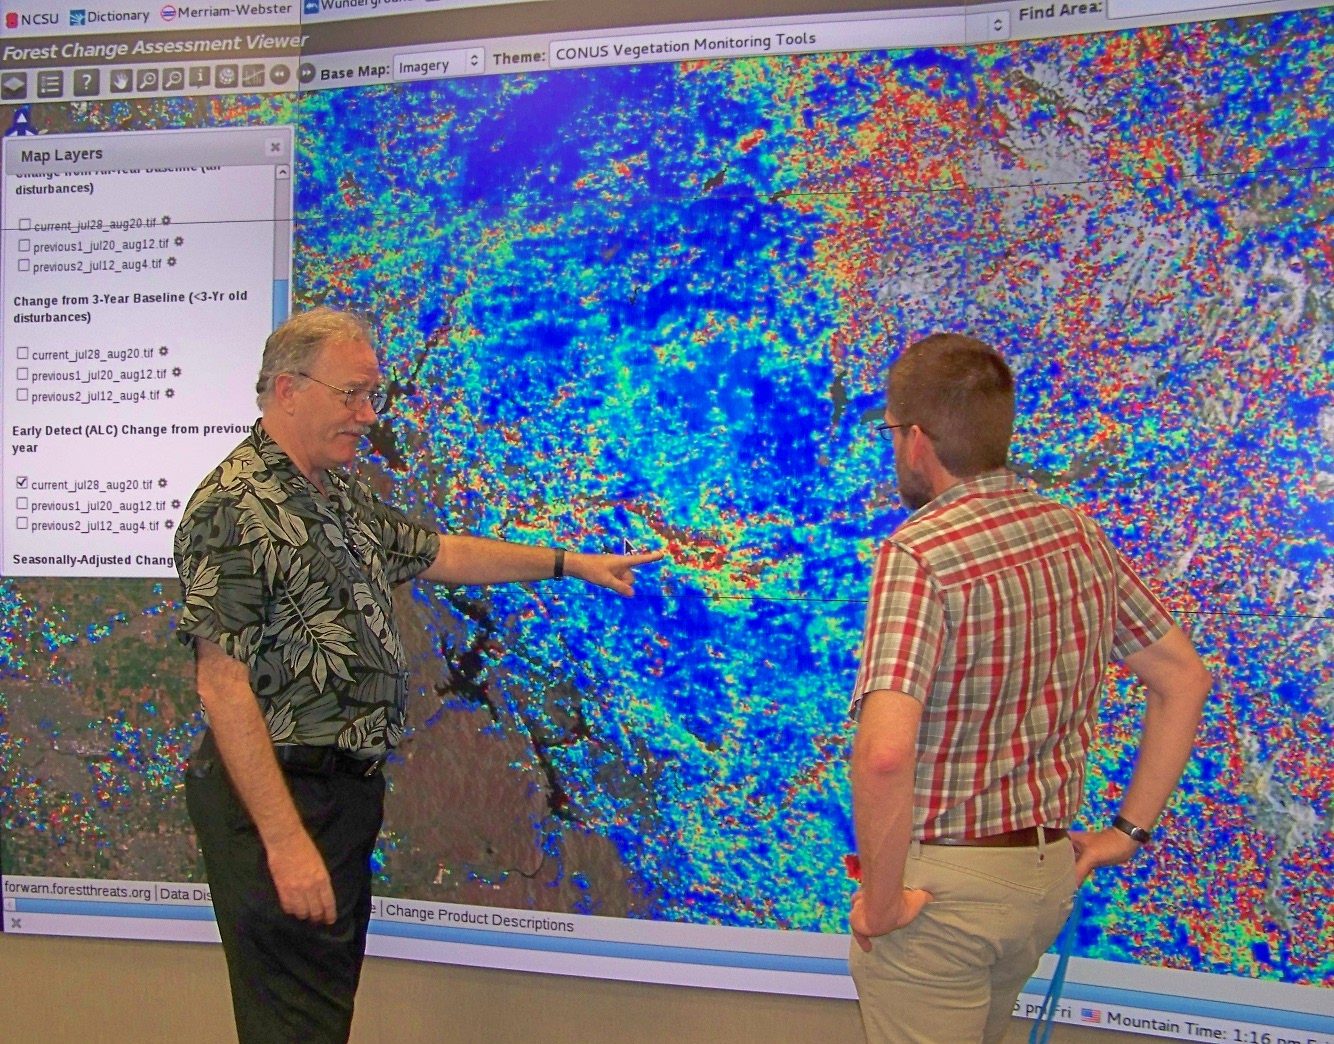
\includegraphics[width=0.94\textwidth]{figures/Hargrove_and_Hoffman_study_the_effects_of_the_growing_Rim_fire_in_California_on_EVEREST_20130823.jpg} \\
%  \href{http://www.ornl.gov/ornl/news/features/2013/forwarn-researchers-get-everest-sized-look-at-woodland-disturbances}{\textit{ForWarn} researchers get EVEREST-sized look at woodland disturbances}
% \end{center}
%\end{frame}
%%%%%%%%%%%%%%%%%%%%%%%%%%%%%%%%%%%%%%%%%%%%%%%%%%%%%%%%%%%%%%%%%%%%%%%%%%%%%%%

%%%%%%%%%%%%%%%%%%%%%%%%%%%%%%%%%%%%%%%%%%%%%%%%%%%%%%%%%%%%%%%%%%%%%%%%%%%%%%%
%\begin{frame}
% \frametitle{Data Mining for Change Detection}
% \begin{itemize}
%  \item Map arithmetic on selected parameters is good for studying the impact of known disturbances, but what is desired is an automated, unsupervised change detection system.
%  \item A data mining approach, utilizing high performance computing (HPC) for the entire body of the very large, high resolution NDVI data history, appears to be the best approach.
%  \item Hoffman and Hargrove previously employed a highly scalable $k$-means algorithm to automatically detect brine scars from hyperspectral remote sensing data~\citep{Hoffman_MS-UTK-Physics_20041104} and for land surface phenology from monthly climatology and 17 years of 8~km NDVI from AVHRR~\citep{White_GRL_20050218}.
%  \item For only the current MODIS NDVI data for 13 years (2000--2012), 46 maps per year, at 250~m over the CONUS, single-precision data exceed 327~GB, requiring HPC resources.
% \end{itemize}
%\end{frame}
%%%%%%%%%%%%%%%%%%%%%%%%%%%%%%%%%%%%%%%%%%%%%%%%%%%%%%%%%%%%%%%%%%%%%%%%%%%%%%%

%%%%%%%%%%%%%%%%%%%%%%%%%%%%%%%%%%%%%%%%%%%%%%%%%%%%%%%%%%%%%%%%%%%%%%%%%%%%%%%
%\begin{frame}
% \frametitle{Geospatiotemporal Data Mining}
% \vskip-0.15in
% \begin{figure}
%  \begin{center}
%   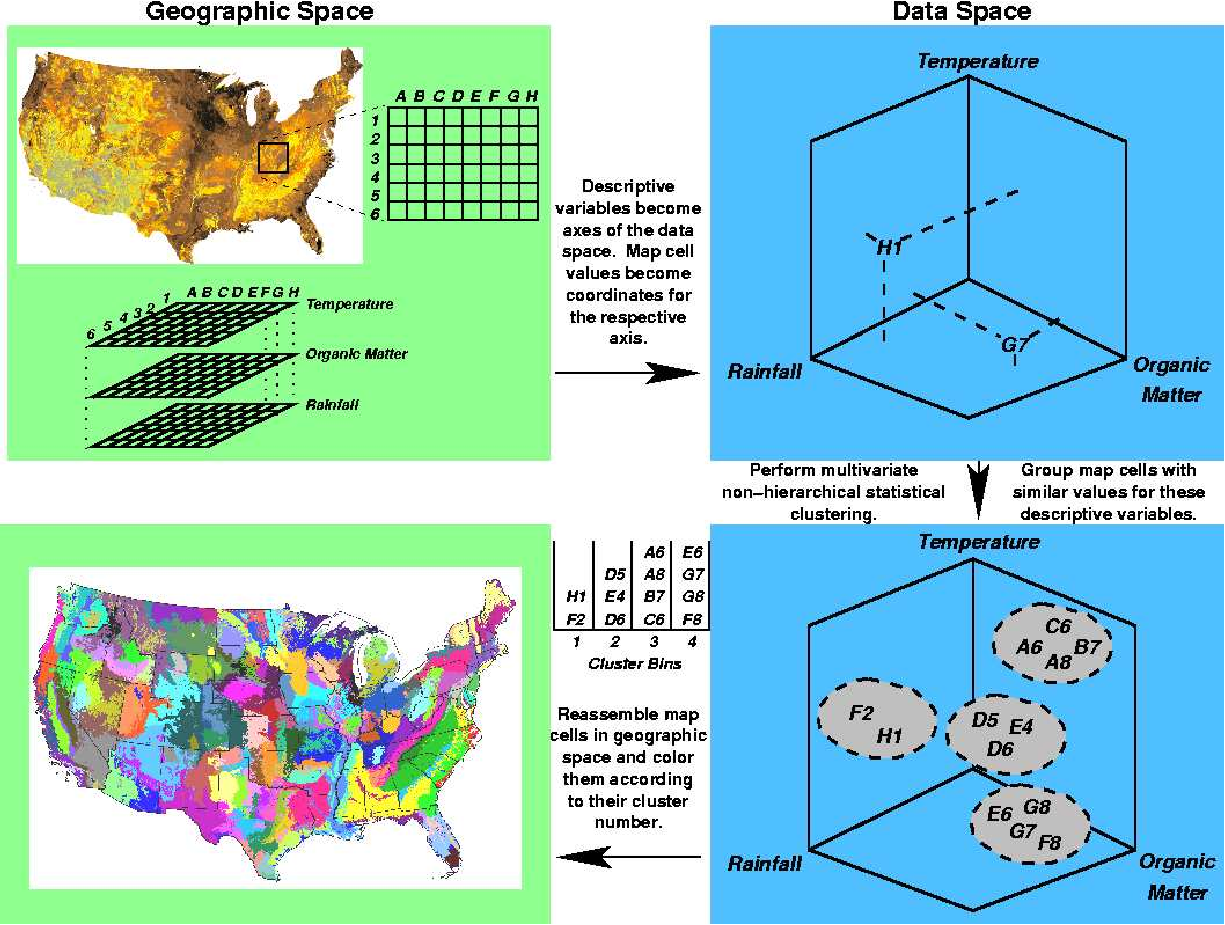
\includegraphics[width=0.91\textwidth]{figures/clusterfinal3}
%  \end{center}
%  %\caption{Cluster analysis.}
%  \label{fig:clusterfinal3}
% \end{figure}
%\end{frame}
%%%%%%%%%%%%%%%%%%%%%%%%%%%%%%%%%%%%%%%%%%%%%%%%%%%%%%%%%%%%%%%%%%%%%%%%%%%%%%%

%%%%%%%%%%%%%%%%%%%%%%%%%%%%%%%%%%%%%%%%%%%%%%%%%%%%%%%%%%%%%%%%%%%%%%%%%%%%%%%
\begin{frame}\small
 \begin{center}
  %\vskip-0.10in
  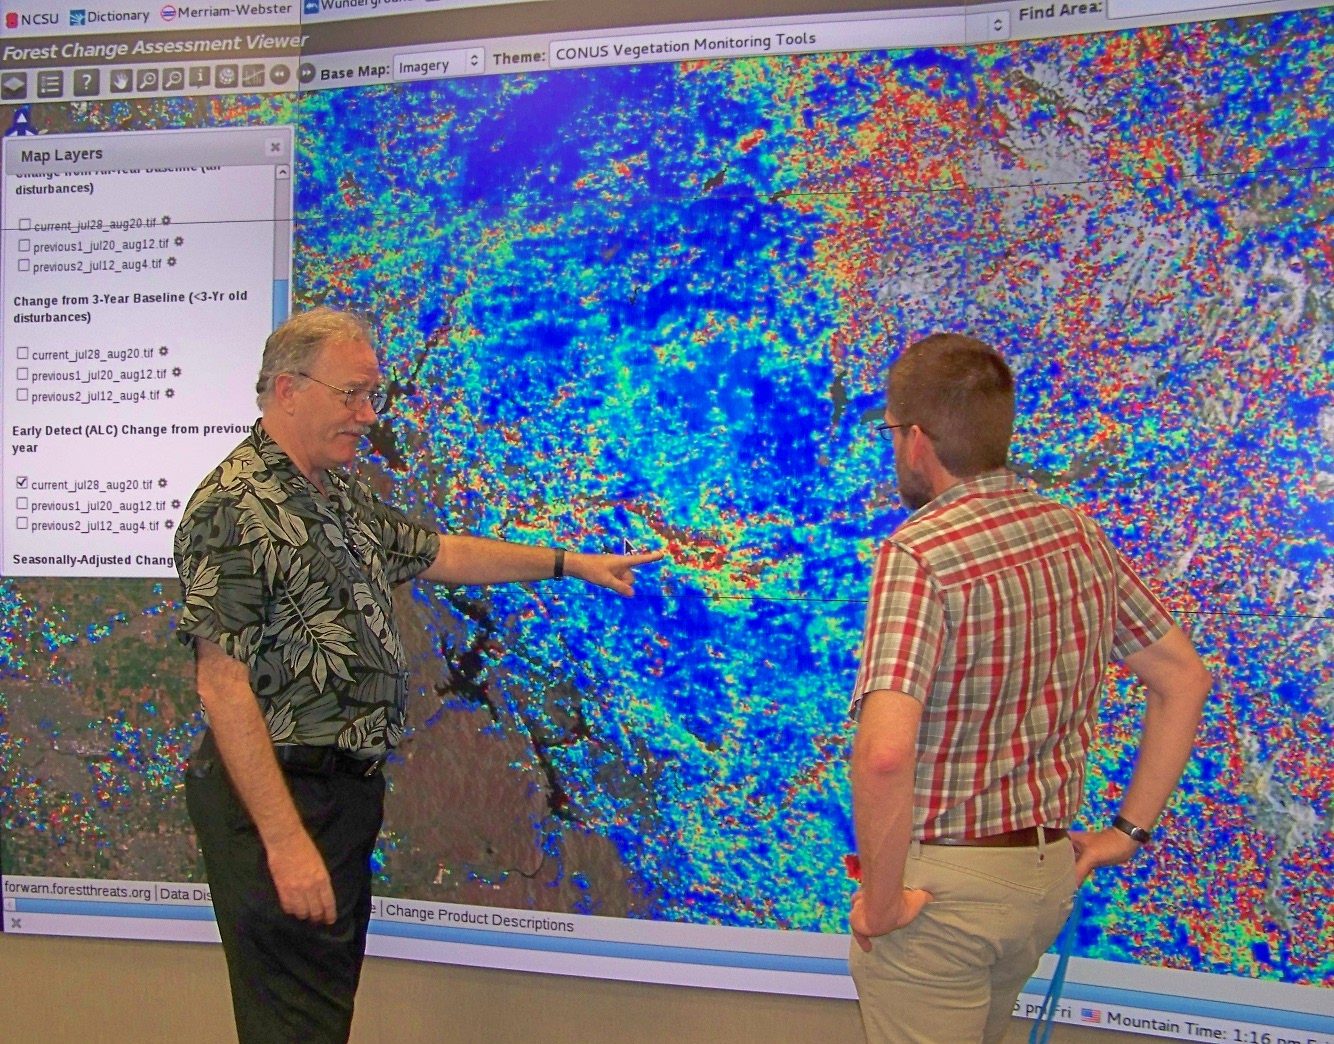
\includegraphics[width=\textwidth]{figures/Hargrove_and_Hoffman_study_the_effects_of_the_growing_Rim_fire_in_California_on_EVEREST_20130823.jpg} \\
  \href{http://www.ornl.gov/ornl/news/features/2013/forwarn-researchers-get-everest-sized-look-at-woodland-disturbances}{\textit{ForWarn} researchers get EVEREST-sized look at woodland disturbances}
 \end{center}
\end{frame}
%%%%%%%%%%%%%%%%%%%%%%%%%%%%%%%%%%%%%%%%%%%%%%%%%%%%%%%%%%%%%%%%%%%%%%%%%%%%%%%

%%%%%%%%%%%%%%%%%%%%%%%%%%%%%%%%%%%%%%%%%%%%%%%%%%%%%%%%%%%%%%%%%%%%%%%%%%%%%%%
\begin{frame}
 \frametitle{\textit{ForWarn} Awards}\scriptsize
 \vskip-0.15in
 \begin{itemize}
  \item \textcolor{blue}{2012 Director's Science Delivery Award} (September 2012) \\
        Dr. Robert Doudrick, Station Director of the USDA Forest Service Southern Research Station
  \item \textcolor{blue}{2013 Interagency Partnership Award} (December 2012) \\
        National Federal Laboratory Consortium (FLC) for Technology Transfer (plus congratulatory letters from \textcolor{red}{Secretary of Energy Ernie Moniz} and \textcolor{red}{Secretary of Agriculture Thomas Vilsack})
  \item \textcolor{blue}{2012 Most Distinguished Scientific or Technical Contribution Award} (December 2012) \\
        ORNL Computer Science \& Mathematics Division (CSMD)
  \item \textcolor{blue}{2012 Partnership Award} (March 2013) \\
        Southeast Regional Federal Laboratory Consortium (FLC) for Technology Transfer
  \item \textcolor{blue}{NASA Group Achievement Award} (August 2013) \\
        Charles Bolden, NASA Administrator
  \item \textcolor{blue}{2013 Southern Research Station Director's Award for Partnerships} (December 2013) \\
        Dr. Robert Doudrick, Station Director of the USDA Forest Service Southern Research Station
  \item \textit{Pending:} \textcolor{blue}{2013 Chief's Honor Award} (March 17, 2014 in Washington, DC) \\
        Thomas L. Tidwell, Chief, USDA Forest Service
 
 \end{itemize}
\end{frame}
%%%%%%%%%%%%%%%%%%%%%%%%%%%%%%%%%%%%%%%%%%%%%%%%%%%%%%%%%%%%%%%%%%%%%%%%%%%%%%%
